%!TEX root = Projeto.tex
\subsection{Fluxos da informação no navegador}

A capacidade que software navegador tem para buscar informação, apresentá-la ao usuário e torná-la interativa é produto da cooperação de subsistemas responsáveis pela comunicação através da rede, a interpretação de código HTML, a representação visual das páginas, o gerenciamento de \textit{caches} e a execução de \scripts{}. O quadro \ref{Fig: diagrama03} ilustra os subsistemas componentes dos navegadores baseados no projeto Chromium \cite{Chromium2018_MPA, Chromium2018_MPRL, HTML5Rocks2011}, enfatizando a hierarquia de componentes desses subsistemas, cujas responsabilidades estão descritas na tabela \ref{table:tabela01}.

\begin{table}
{\small\renewcommand{\arraystretch}{1.5}
	\begin{tabularx}{\textwidth}{|l|X|}
		\hline 
		\textbf{Subsistema} & \textbf{Responsabilidade} \\ 
		\hline 
		\textbf{Interface do usuário} & Expor os elementos interativos de que o usuário dispõe para comandar o navegador, como a barra de endereços, os comandos de navegação (``voltar'', ``avançar'', ``recarregar'') e os comandos de menu do navegador, incluindo os menus de contexto, atalhos, acesso às configurações e às extensões. A janela de interface do usuário hospeda, ainda, o componente de superfície (\textit{canvas}) responsável pela exibição do conteúdo tornado visível (``renderizado'') pelo subsistema Mecanismo do navegador.\\ 
		\hline 
		\textbf{Mecanismo do navegador} & Comandar o mecanismo de visualização sob a demanda das ações originadas pela interface do usuário e, em resposta a esses comandos, sinalizar mudanças de estado que serão refletidas pela interface de usuário. Exemplo disso é o ciclo de carregamento de páginas da web, que dispara o \textit{download} de recursos de rede, a renderização desses recursos e a atualização da interface de usuário à medida em que as etapas do carregamento se sucedem.\\ 
		\hline
		\textbf{Mecanismo de visualização} & ``Renderizar'', ou transformar em conteúdo audiovisual, o fluxo de dados transferidos pelo subsistema de acesso à rede. O fluxo de dados carrega informação textual codificada nas linguagens HTML e CSS, e também dados binários em formato de imagem, áudio e vídeo. O mecanismo de visualização pode dar suporte à renderização de dados em formatos não vinculados à HTML, como documentos PDF e arquivos XML.\\
		\hline
		\textbf{Acesso à rede} & Conectar-se aos provedores de informação indicados por meio de URLs (\textit{uniform resource locators}) e estabelecer fluxos de dados sob diferentes protocolos como HTTP, HTTPS, Web Sockets, WebRTC e FTP.\\
		\hline
		\textbf{Persistência de dados} & Prover funcionalidades para armazenamento de dados persistentes, incluindo \textit{caches}, \textit{cookies}, suporte ao sistema de arquivos e as APIs para bancos de dados de escala reduzida como \textit{localStorage} e IndexedDB.\\
		\hline
		\textbf{Interpretador de Javascript} & Compilar e executar código na linguagem Javascript. ``V8'', ``Chakra'' e ``SpiderMonkey'' são os nomes dos subsistemas de interpretação de Javascript empregados pelos navegadores Chrome, Microsoft Edge e Firefox, respectivamente. Os diversos interpretadores aderem às especificações estabelecidas pelo consórcio ECMA sob o padrão ``ECMAScript'', que define a sintaxe e os recursos que devem ser suportados pela linguagem.\\
		\hline
	\end{tabularx}
}
\caption{Responsabilidades dos subsistemas do navegador}
\label{table:tabela01}
\end{table}

%As responsabilidades desses subsistemas são segregadas entre processos distintos, o que eleva a capacidade do navegador de se manter funcional mesmo quando uma determinada página provoca uma falha de execução que termina seu processo hospedeiro \dubious{(e falta ilustrar essa segregação)}

\begin{figure}[h]
	\centering
	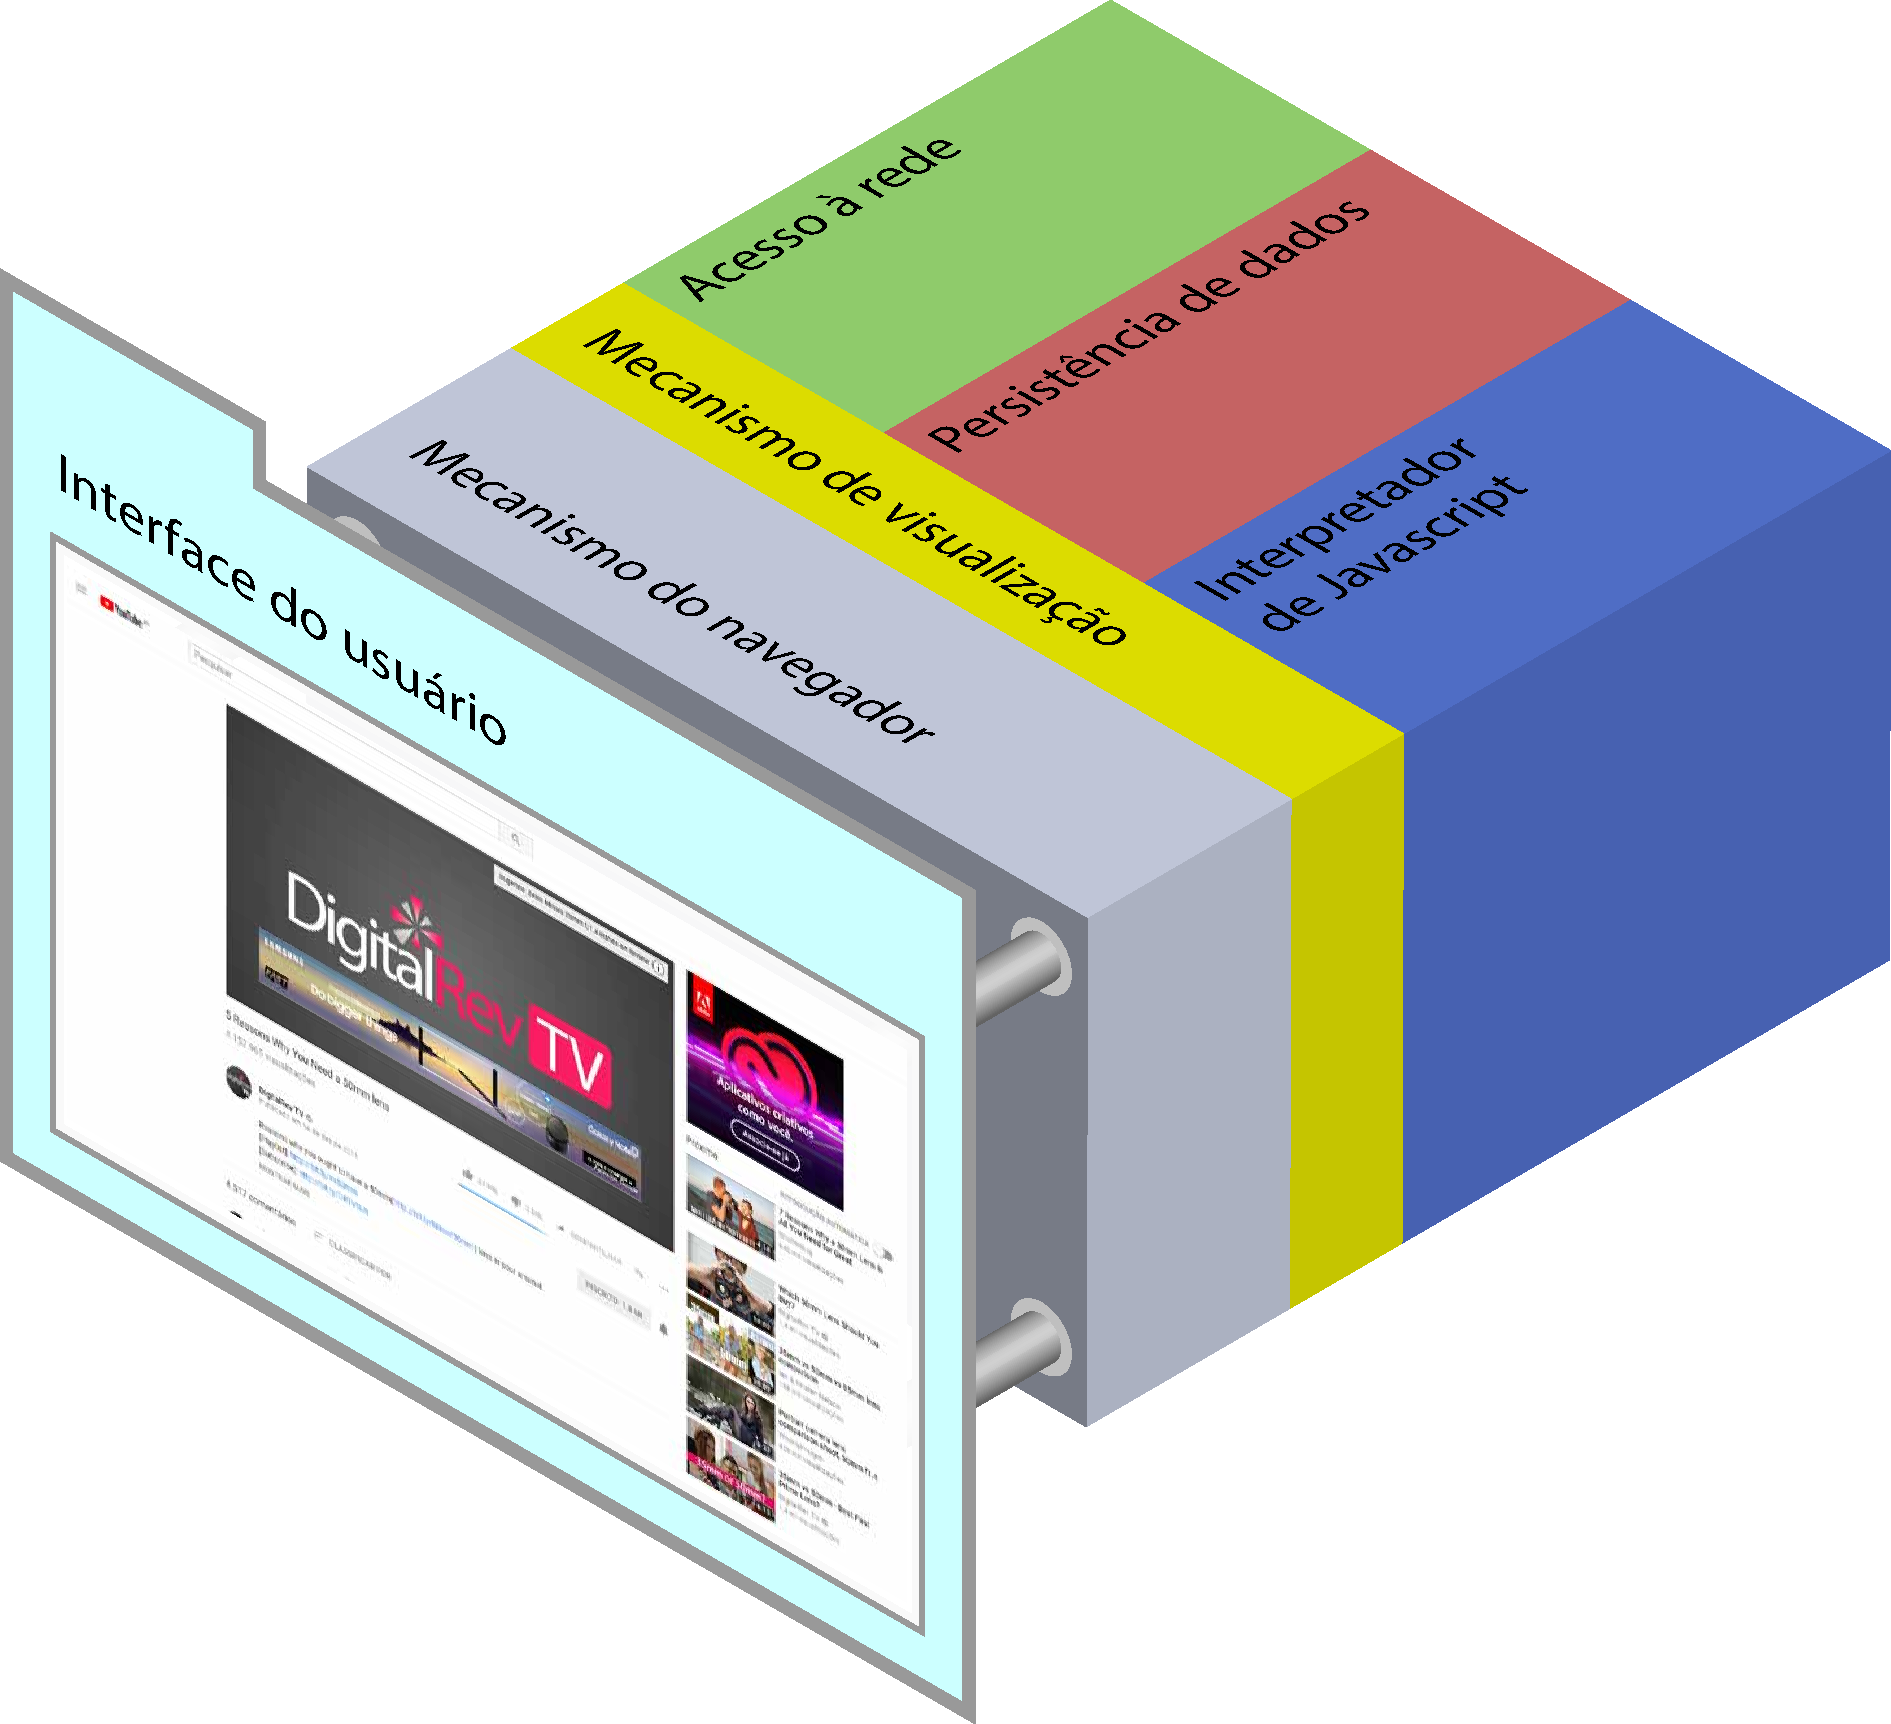
\includegraphics[width=12cm]{diagramas/diagrama03.pdf}
	\label{Fig: diagrama03}
	\caption{Componentes do navegador de código aberto Chromium}
\end{figure}

Sob o ponto de vista da segurança da informação, cabem algumas observações:

\begin{alineas}
	\item Os subsistemas do navegador podem apresentar conjuntos próprios de vulnerabilidades, inerentes ao funcionamento e à implementação de cada um;
	\item O inter-relacionamento entre esses subsistemas estabelece fluxos de informação que, por sua vez, também podem apresentar vulnerabilidades;
	\item Ao longo do tempo, a descoberta de vulnerabilidades e a evolução dos navegadores contribuíram para o estabelecimento de políticas para a segurança na web;
	\item A manutenção de certas funcionalidades, necessárias para o funcionamento das aplicações web modernas, comprometeu a capacidade do navegador de se manter imune a todas as vulnerabilidades de vazamento de informação possíveis.
\end{alineas}

\subsubsection{Ciclo de vida de uma página da web}

O ciclo de vida de uma página da web é a sequência de atividades executadas pelo navegador durante os processos de carga, exibição e  interação do usuário com o conteúdo visualizado, perdurando até a ação de descarregamento da página, desencadeada pela navegação do usuário ou pelo encerramento do programa navegador. A informação mantida ou criada dentro do ciclo de vida de uma página tende a ser volátil, sendo descartada no descarregamento a menos que seja transmitida para outro \textit{host} ou armazenada localmente em estruturas como \textit{localStorage} e IndexedDB.

\begin{todo}
Pontos a considerar:

\begin{alineas}
	\item O navegador da web é um cliente da internet.
	\item O ciclo de vida de uma página é "curto" (cada página, uma aplicação diferente? um contexto de execução diferente?)
	\item Onde está a informação no navegador, e qual sua duração possível?
	\begin{alineas}
		\item Endereço (URL) corrente
		\item Requisição (pode ser da página como de "sub-recursos" como imagens, iframes, scripts, estilos, xhr...)
		\item Resposta
		\item Estrutura da página (DOM)
		\item Eventos do navegador/DOM
		\item Closures
		\item Pilha de chamadas
		\item Extensões do navegador
		\item Caches
		\item Cookies
		\item Local DB
		\item Em HTTPS, temos mais fluxos?
	\end{alineas}
\end{alineas}

Então será possível indicar quais dos fluxos estão protegidos contra vazamento de informação, e como estão. E consequentemente quais fluxos não estão cobertos.
\end{todo}
